\documentclass{article}
\usepackage[utf8]{inputenc}
\usepackage{graphicx}
\usepackage[font=small,labelfont=bf]{caption}

\title{Edit Distance con e Senza N-Grams}
\author{Mirko Bicchierai }
\date{June 2021}

\begin{document}

\maketitle

\section{Analisi Teorica}
\subsection{Edit Distance}
L'Edit Distance è un algoritmo di programmazione dinamica che consente di trovare, dato un set di operazioni con dei costi, il minor costo di trasformazione di una parola $x$ in un'altra $y$.
\paragraph{Operazioni}
\subparagraph{Copia}Il carattere viene mantenuto, ha costo 0.
\subparagraph{Sostituzione} Si sostituisce un carattere con un altro, ha costo 1.
\subparagraph{Cancellazione} Si elimina un carattere, ha costo 1.
\subparagraph{Inserimento} Si inserisce un carattere, ha costo 1.
\subparagraph{Scambio} Si invertono due caratteri adiacenti, è una combinazione delle altre, ha costo 1.

\paragraph{Pseudocodice}
\begin{verbatim}
Edit-Distance(x, y)
begin
    m:=x.lenght
    n:=y.lenght
    
    for i:=0 to m
    begin
        c[i][]0]:=i*cost(CANCELLAZIONE)
    end

    for i:=0 to n
    begin
        c[0][i]:=i*cost(INSERIMENTO)
    end
    
    for i:=1 to m
    begin
        for i:=1 to m
        begin
            c[i][j]:=Infinity
            if x[i]=y[j] then
            begin
                c[i][j]=c[i-1][j-1]+cost(COPIA)
            end
            if (x[i]<>y[j]) AND (c[i-1][j-1]+cost(SOSTITUZIONE)<c[i][j]) then
            begin
                c[i][j]=c[i-1][j-1]+cost(SOSTITUZIONE)
            end
            if (i>=2) AND (j>=2) AND (x[i-1]=y[j]) AND (y[i-1]=x[j]) 
                AND (c[i-2][j-2]+cost(SCAMBIO)<c[i][j]) then
            begin
                c[i][j]=c[i-2][j-2]+cost(SCAMBIO)
            end
            if c[i-1][j]+cost(CANCELLAZIONE)<c[i][j] then
            begin
                c[i][j]=c[i-1][j]+cost(CANCELLAZIONE)
            end
            if c[i][j-1]+cost(INSERIMENTO)<c[i][j] then
            begin
                c[i][j]=c[i][j-1]+cost(INSERIMENTO)
            end
        end
    end
    return C
end
\end{verbatim}
\paragraph{Utilizzo}
L'edit distance è usato per la correzzione ortografica in vari ambiti, ad esempio nelle ricerche su Google o nella correzione delle letture degli OCR. Ci sono principalmente due approcci possibili nel suo utilizzo: {\itshape Context-Sensitive} in questo caso non si va ad analizzare solo la parola ma anche il contesto in cui è scritta, questo approcio risulta più accurato ma è anche più complesso; {\itshape Parole Isolate}, in questo caso si considera soltanto la parola estrapolata dal contesto in cui è scritta.
\subparagraph{Edit Distance in un Lessico}
Spesso è necessario avere un lessico, o una collezione di parole, di riferimento nel quale trovare la parola "più vicina" a quella data. Utilizzando la normale edit distance è molto costoso, poichè si deve confrontare con tutte le parole; in questo caso si utilizza un approccio particolare: si calcolano tutte le permutazioni possibili della parola data con un costo inferiore ad un soglia, quindi si fa l'intersezione tra questo insieme ed il lessico.
Fare questa operazione non è sempre conveniente, si usano quindi delle varianti dell'algoritmno: {\itshape Weighted Edit Distance} e {\itshape Intersezione N-Gram}. 
\subsection{Weighted Edit Distance}
In questa variante il costo delle operazioni non dipende solo dalla sua tipologia, ma anche dai caratteri coinvolti, questo aiuta ad adattare l'algoritmo al contesto nel quale viene utilizzato: se è implementato in un motore di ricerca è logico attribuire un costo minore alla sostituzione tra due lettere adiacenti nella tastiera o all'inserimento; al contrario un approccio simile nel caso di correzione del testo di un OCR sarebbe insensato; risulta più opportuno considerare un costo di scambio minore tra lettere che vengono facilmente confuse dal riconoscitore.
\subsection{Intersezione N-Gram}
Questo approccio aiuta a diminuire il numero di parole da confrontare con edit distance, si usano gli n-grams che sono tutti sottoinsiemi possibili di n lettere consecutive all'interno di una parola. Confrontando gli n-grams della parola data con quelli dei vocaboli nel lessico possiamo definire un modo per stabilire se ha senso eseguire edit distance.
Per avere una misura normalizzata di questa "somiglianza" tra le parole si usa il {\itshape Coefficiente di Jaccard}.
\paragraph{Coefficiente di Jaccard} Il Coefficente di Jaccard fornisce una misura della similarità tra due insiemi, il coefficiente ha valore tra 0 e 1, se è 1 gli insiemi sono identici.
Si calcola:  $JC=\frac{X\cap Y}{X\cup Y}$.

Nel caso che prendiamo in considerazione gli insiemi sono gli n-grams, una soglia di similarità accettabile è quella in cui $JC \geq 0,8$

\section{Confronto Tra Edit Distance Con e Senza N-Grams}
\paragraph{Descrizione Test}
L'esperimento consiste nell'esecuzione dell'algoritmo edit distance con e senza l'intersezione N-Gram, sarà testato con alcuni dizionario italiani, verranno riportati i rusultati per il dizionario di 60000 parole ed il dizionario da 95000 parole. Saranno proposte varie grandezze di N-Grams: 2, 3, 4 e 5-Grams, per verificare le differenze di velocità di esecuzione al variare della dimesione.

Di seguito sono proposti 5 tipi di test nei quali varierà il tipo di input agli algoritmi: una parola del dizionario, una parola con due lettere invertite, una parola con una lettera aggiunta, una parola con una lettera tolta e una parola che non appartiene al dizionario.
\paragraph{Aspettative}
Analizzando la teoria il risultato dell'
esperimento appare scontato, poiche l'esecuzione di edit distance senza intersezione N-Gram confronta ogni singola parola del dizionario; anche quelle che risultano decisamente diverse dalla parola considerata. Possiamo usare questo test per evidenziare anche la differenza di velocita al variare della grandezza dell'N-Gram.
\subsection{Parola Del Dizionario}
\subsubsection{60000}
Di seguito i tempi di esecuzione degli algoritmi sul dizionario di 60000 parole:
\medskip

\begin{tabular}{ |p{3cm}||p{3.5cm}|  }
 \hline
 \multicolumn{2}{|c|}{Tempo Con Una Parola Appartenente Al Dizionario} \\
\hline
 Senza N-Gram  &   3.78594\\\hline
 2-Gram &  0.16309    \\\hline
 3-Gram & 0.14349 \\\hline
 4-Gram & 0.11983\\\hline
 5-Gram & 0.10329  \\
 \hline
\end{tabular}

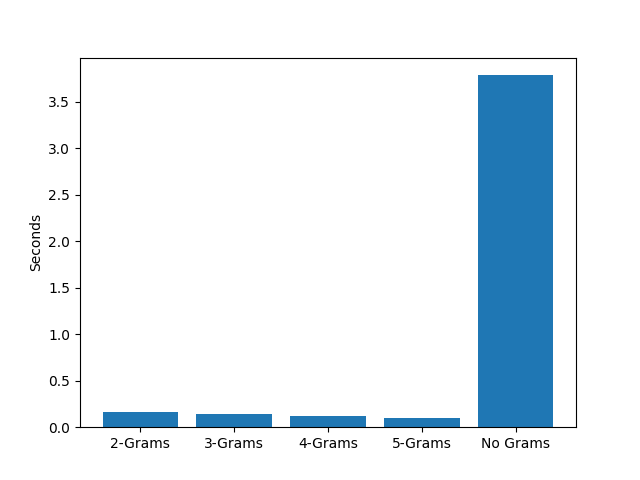
\includegraphics[scale=0.5]{img/ParolaNonModificata_60000_parole.png}
\captionof{figure}{Tempi Con Una Parola nel Dizionario}

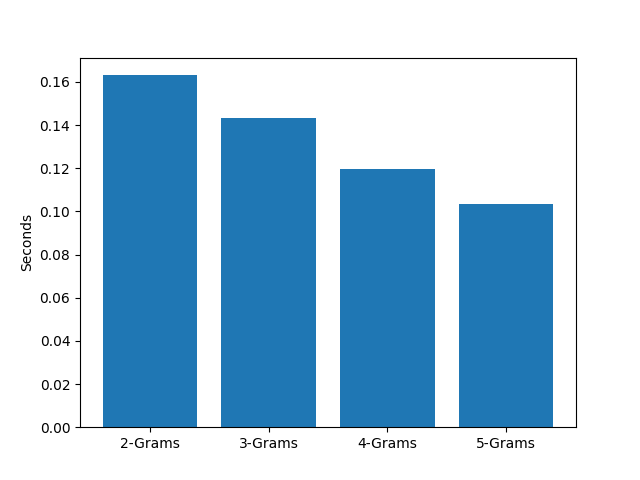
\includegraphics[scale=0.5]{img/ParolaNonModificataSoloGram_60000_parole.png}
\captionof{figure}{Tempi Con Una Parola nel Dizionario, Confronto Tra N-Grams}
\subsubsection{95000}
Di seguito i tempi di esecuzione degli algoritmi sul dizionario di 95000 parole:
\medskip

\begin{tabular}{ |p{3cm}||p{3.5cm}|  }
 \hline
 \multicolumn{2}{|c|}{Tempo Con Una Parola Appartenente Al Dizionario} \\
\hline
 Senza N-Gram  &   7.01881\\\hline
 2-Gram &  0.28797   \\\hline
 3-Gram & 0.2516 \\\hline
 4-Gram & 0.21814\\\hline
 5-Gram & 0.18551  \\
 \hline
\end{tabular}

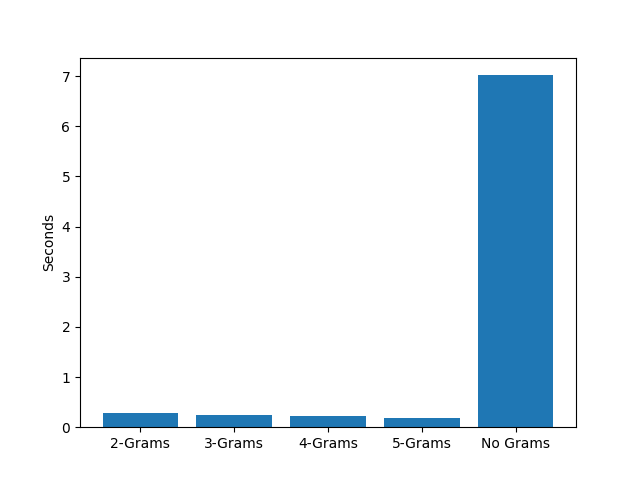
\includegraphics[scale=0.5]{img/ParolaNonModificata_95000_parole.png}
\captionof{figure}{Tempi Con Una Parola nel Dizionario}

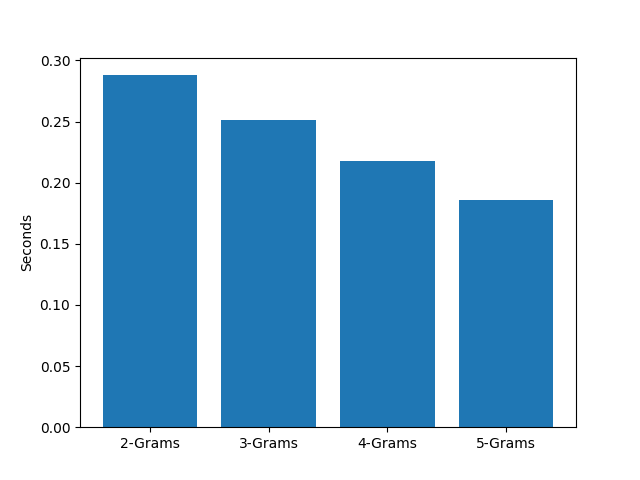
\includegraphics[scale=0.5]{img/ParolaNonModificataSoloGram_95000_parole.png}
\captionof{figure}{Tempi Con Una Parola nel Dizionario, Confronto Tra N-Grams}


\subsection{Parola Con Lettere Scambiate}
\subsubsection{60000}
Di seguito i tempi di esecuzione degli algoritmi:
\medskip

\begin{tabular}{ |p{3cm}||p{3.5cm}|  }
 \hline
 \multicolumn{2}{|c|}{Tempo Con Una Parola Con Lettere Scambiate} \\
\hline
 Senza N-Gram  &   3.65345\\\hline
 2-Gram &  0.1622    \\\hline
 3-Gram & 0.13885 \\\hline
 4-Gram & 0.1218\\\hline
 5-Gram & 0.10255  \\
 \hline
\end{tabular}

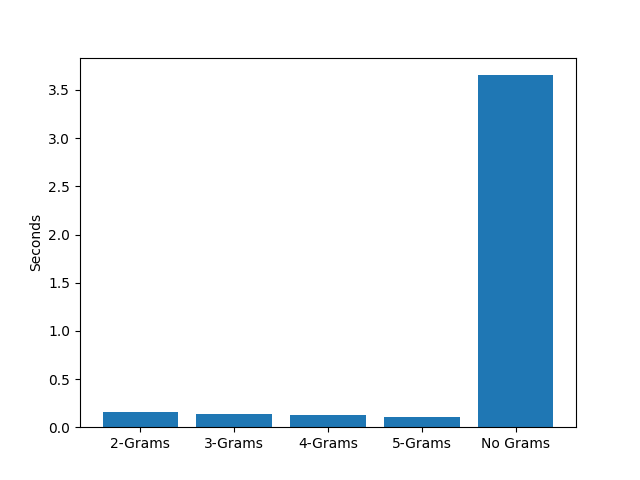
\includegraphics[scale=0.5]{img/LetteraScambiata_60000_parole.png}
\captionof{figure}{Tempi con una parola con due lettere scambiate}

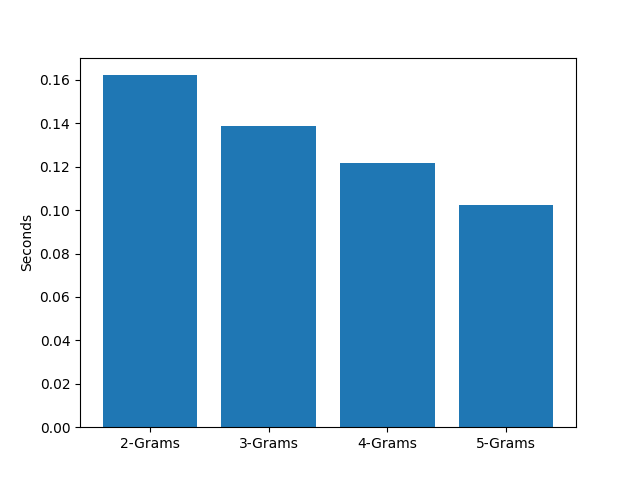
\includegraphics[scale=0.5]{img/LetteraScambiataSoloGram_60000_parole.png}
\captionof{figure}{Tempi con una parola con due lettere scambiate, confronto tra N-Grams}

\subsubsection{95000}
Di seguito i tempi di esecuzione degli algoritmi sul dizionario di 95000 parole:
\medskip

\begin{tabular}{ |p{3cm}||p{3.5cm}|  }
 \hline
 \multicolumn{2}{|c|}{Tempo Con Una Parola Con Lettere Scambiate} \\
\hline
 Senza N-Gram  &   6.6963\\\hline
 2-Gram &  0.29016   \\\hline
 3-Gram & 0.25864 \\\hline
 4-Gram & 0.21948\\\hline
 5-Gram & 0.19081  \\
 \hline
\end{tabular}

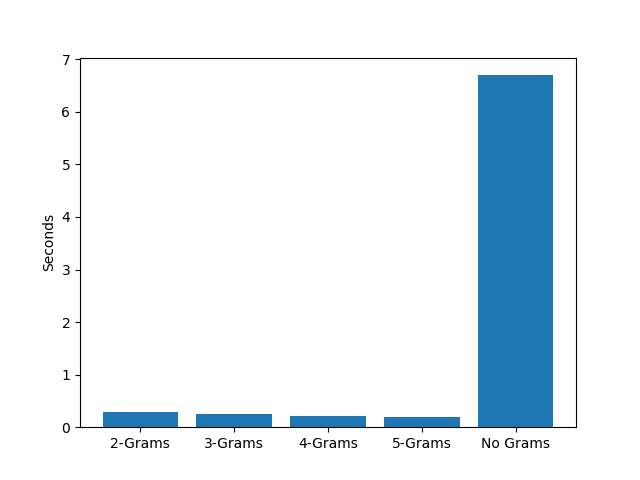
\includegraphics[scale=0.5]{img/LetteraScambiata_95000_parole.png}
\captionof{figure}{Tempi con una parola con due lettere scambiate}

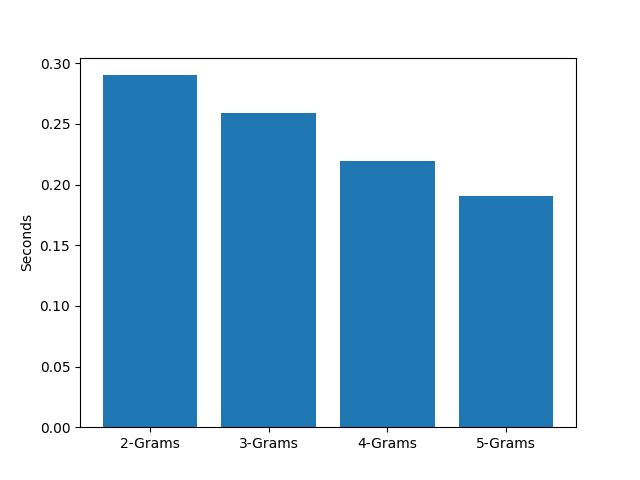
\includegraphics[scale=0.5]{img/LetteraScambiataSoloGram_95000_parole.png}
\captionof{figure}{Tempi con una parola con due lettere scambiate, confronto tra N-Grams}


\subsection{Parola Con Una Lettera Aggiunta}
\subsubsection{60000}
Di seguito i tempi di esecuzione degli algoritmi:
\medskip

\begin{tabular}{ |p{3cm}||p{3.5cm}|  }
 \hline
 \multicolumn{2}{|c|}{Tempo Con Una Parola Con Una Lettera Aggiunta} \\
\hline
 Senza N-Gram  &   4.20403\\\hline
 2-Gram &  0.17107    \\\hline
 3-Gram & 0.14739 \\\hline
 4-Gram & 0.12623\\\hline
 5-Gram & 0.10807  \\
 \hline
\end{tabular}

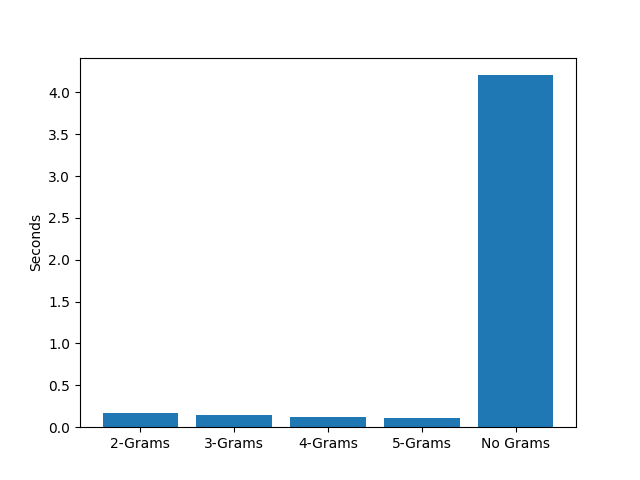
\includegraphics[scale=0.5]{img/LetteraAggiunta_60000_parole.png}
\captionof{figure}{Tempi con una parola con una Lettera Aggiunta}


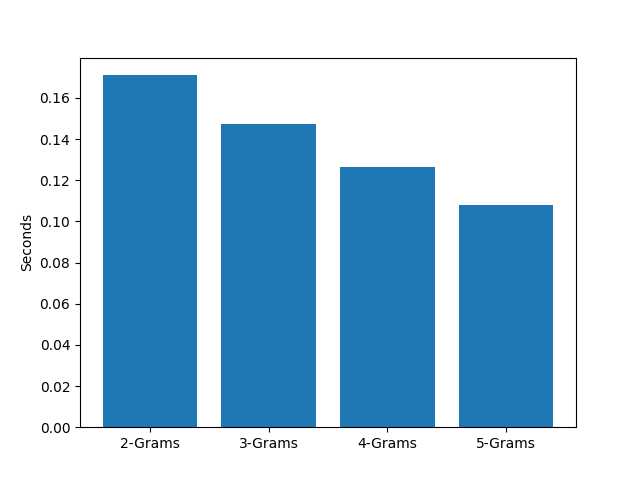
\includegraphics[scale=0.5]{img/LetteraAggiuntaSoloGram_60000_parole.png}
\captionof{figure}{Tempi con una parola con una Lettera Aggiunta, Confronto Tra N-Grams}

\subsubsection{95000}
Di seguito i tempi di esecuzione degli algoritmi sul dizionario di 95000 parole:
\medskip

\begin{tabular}{ |p{3cm}||p{3.5cm}|  }
 \hline
 \multicolumn{2}{|c|}{Tempo Con Una Parola Con Una Lettera Aggiunta} \\
\hline
 Senza N-Gram  &  7.65363\\\hline
 2-Gram &  0.30946   \\\hline
 3-Gram & 0.26979 \\\hline
 4-Gram & 0.23365\\\hline
 5-Gram & 0.20293  \\
 \hline
\end{tabular}

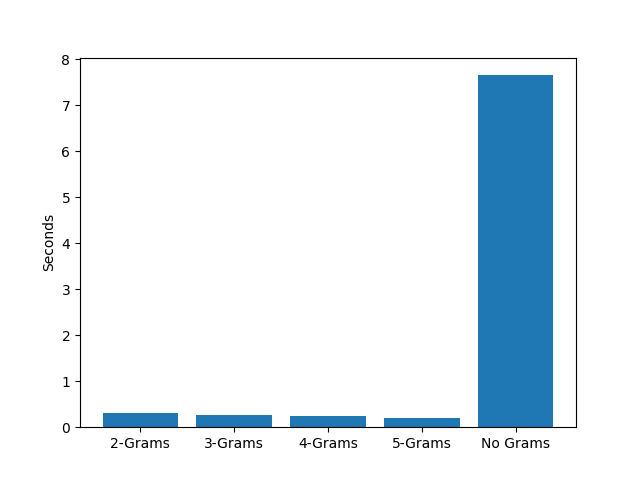
\includegraphics[scale=0.5]{img/LetteraAggiunta_95000_parole.png}
\captionof{figure}{Tempi con una parola con una Lettera Aggiunta}

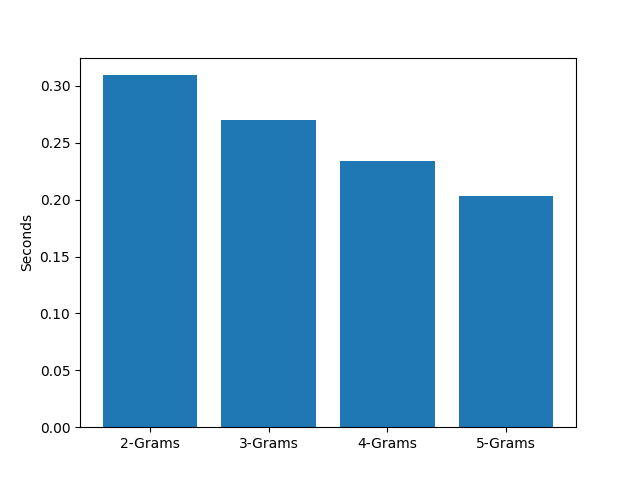
\includegraphics[scale=0.5]{img/LetteraAggiuntaSoloGram_95000_parole.png}
\captionof{figure}{Tempi con una parola con una Lettera Aggiunta, Confronto Tra N-Grams}


\subsection{Parola Con Una Lettera Rimossa}
\subsubsection{60000}
Di seguito i tempi di esecuzione degli algoritmi:
\medskip

\begin{tabular}{ |p{3cm}||p{3.5cm}|  }
 \hline
 \multicolumn{2}{|c|}{Tempo Con Una Parola Con Una Lettera Rimossa} \\
\hline
 Senza N-Gram  &   3.26765\\\hline
 2-Gram &  0.15186    \\\hline
 3-Gram & 0.13134 \\\hline
 4-Gram & 0.11655\\\hline
 5-Gram & 0.09695  \\
 \hline
\end{tabular}

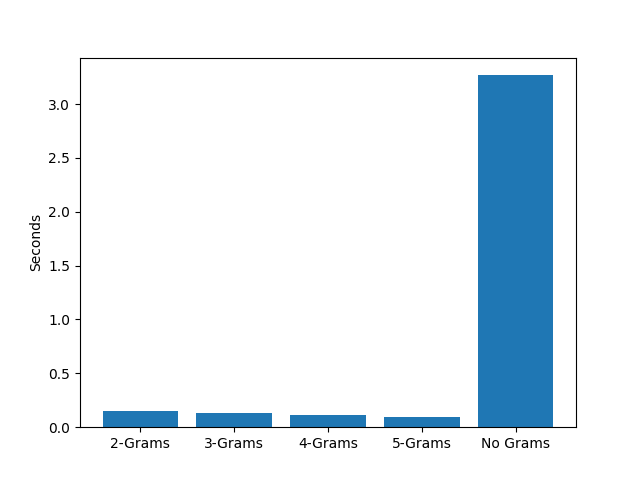
\includegraphics[scale=0.5]{img/LetteraRimossa_60000_parole.png}
\captionof{figure}{Tempi con una parola con una lettera rimossa}

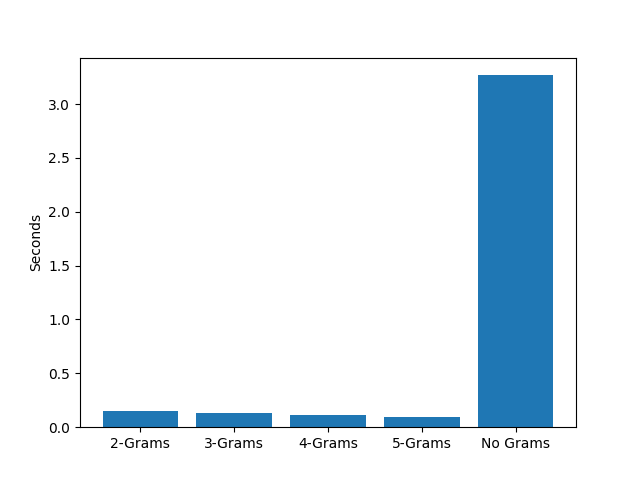
\includegraphics[scale=0.5]{img/LetteraRimossa_60000_parole.png}
\captionof{figure}{Tempi con una parola con una lettera rimossa, confronto tra N-Grams}

\subsubsection{95000}
Di seguito i tempi di esecuzione degli algoritmi sul dizionario di 95000 parole:
\medskip

\begin{tabular}{ |p{3cm}||p{3.5cm}|  }
 \hline
 \multicolumn{2}{|c|}{Tempo Con Una Parola Con Una Lettera Rimossa} \\
\hline
 Senza N-Gram  &   6.6472\\\hline
 2-Gram &  0.34086  \\\hline
 3-Gram & 0.29199 \\\hline
 4-Gram & 0.2672\\\hline
 5-Gram & 0.17287  \\
 \hline
\end{tabular}

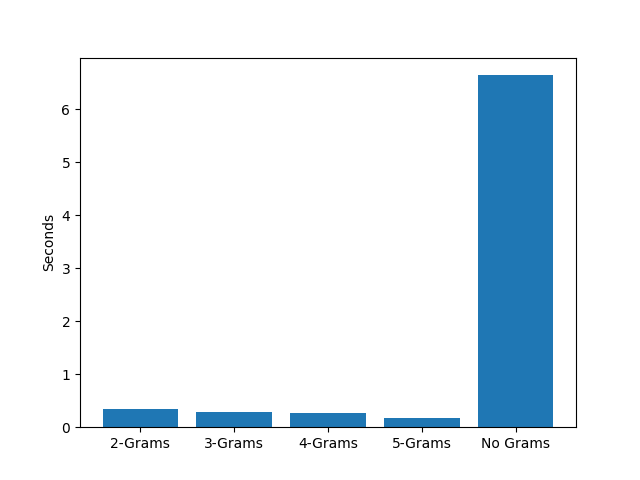
\includegraphics[scale=0.5]{img/LetteraRimossa_95000_parole.png}
\captionof{figure}{Tempi con una parola con una lettera rimossa}

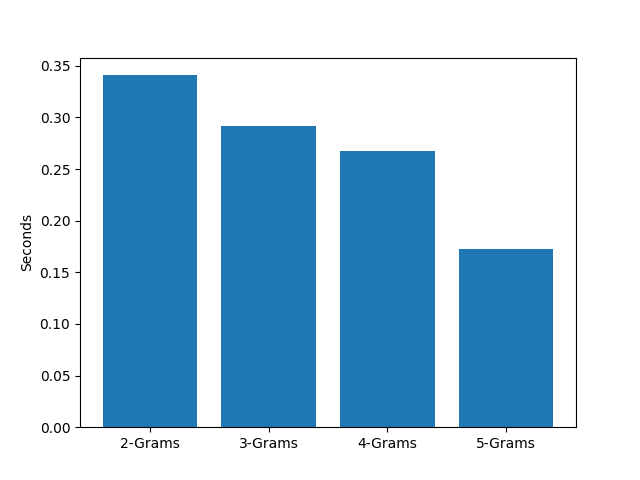
\includegraphics[scale=0.5]{img/LetteraRimossaSoloGram_95000_parole.png}
\captionof{figure}{Tempi con una parola con una lettera rimossa, confronto tra N-Grams}

\subsection{Parola Non Appartenente Al Dizionario}
\subsubsection{60000}
Di seguito i tempi di esecuzione degli algoritmi:
\medskip

\begin{tabular}{ |p{3cm}||p{3.5cm}|  }
 \hline
 \multicolumn{2}{|c|}{Tempo Con Una Parola Non Appartenente Al Dizionario} \\
\hline
 Senza N-Gram  &   5.98974\\
 \hline
 2-Gram &  0.19202    \\\hline
 3-Gram & 0.1678 \\\hline
 4-Gram & 0.14407\\\hline
 5-Gram & 0.12129  \\
 \hline
\end{tabular}


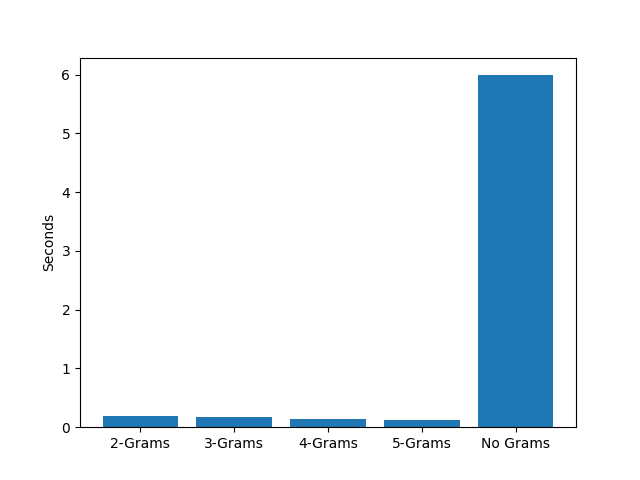
\includegraphics[scale=0.5]{img/ParolaNonAppartenente60000_parole.png}
\captionof{figure}{Tempi Con Una Parola }

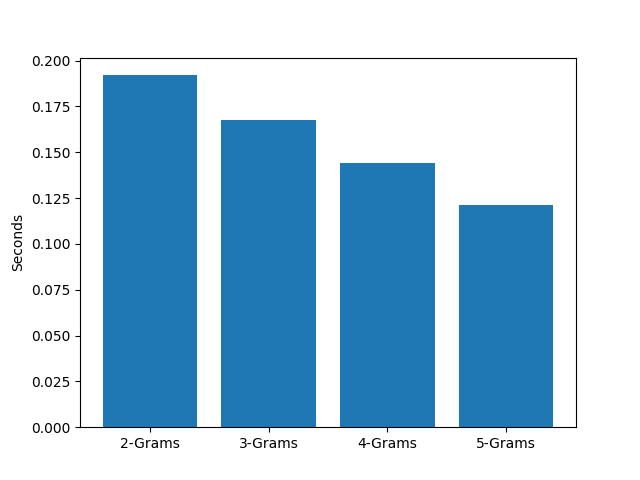
\includegraphics[scale=0.5]{img/ParolaNonAppartenenteSoloGram60000_parole.png}
\captionof{figure}{Tempi Con Una Parola, Confronto Tra Gli N-Grams }

\subsubsection{95000}
Di seguito i tempi di esecuzione degli algoritmi sul dizionario di 95000 parole:
\medskip

\begin{tabular}{ |p{3cm}||p{3.5cm}|  }
 \hline
 \multicolumn{2}{|c|}{Tempo Con Una Parola Non Appartenente Al Dizionario} \\
\hline
 Senza N-Gram  &   12.15947\\\hline
 2-Gram &  0.35214   \\\hline
 3-Gram & 0.35214\\\hline
 4-Gram & 0.27089\\\hline
 5-Gram & 0.23165  \\
 \hline
\end{tabular}

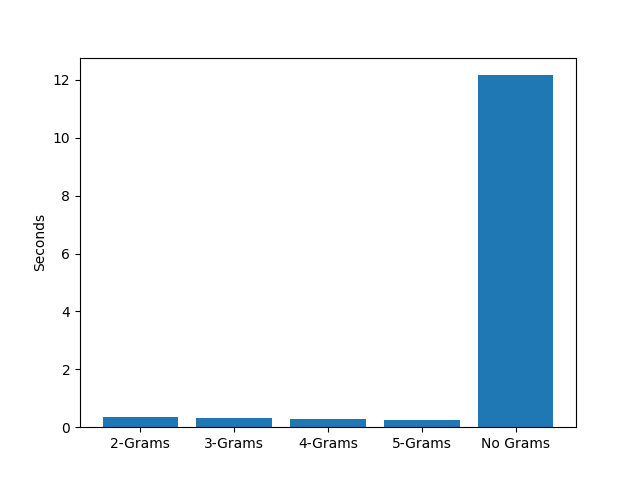
\includegraphics[scale=0.5]{img/ParolaNonAppartenente95000_parole.png}
\captionof{figure}{Tempi Con Una Parola}

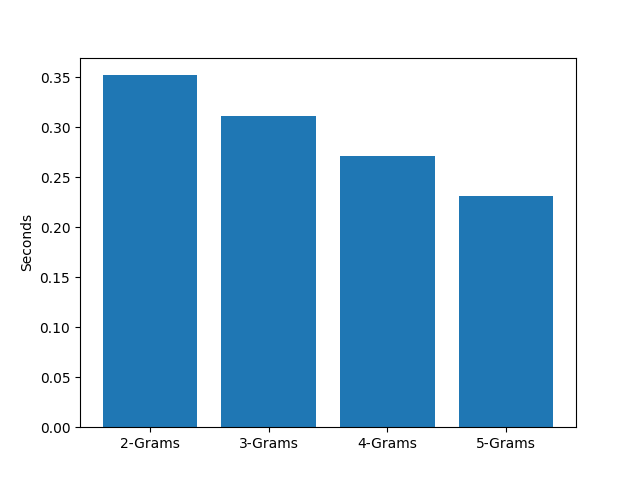
\includegraphics[scale=0.5]{img/ParolaNonAppartenenteSoloGram95000_parole.png}
\captionof{figure}{Tempi Con Una Parola, Confronto Tra Gli N-Grams}


\section{Conclusioni}
Come previsto la differenza di velocità di esecuzione tra i due diversi approcci risulta abissale, ciò è dovuto all'analisi degli N-Grams che grazie al coefficiente di Jaquart permettono di escludere le parole che non sono minimamente simili a quella che stiamo considerando.

La grandezza dell'N-Gram influisce in maniera marginale rispetto all'esecuzione senza di esso; possiamo notare che in quasi tutti i casi aumentando la grandezza dell'N-Gram diminuiscono anche i tempi di esecuzione. 
\end{document}